%%%%%%%%%%%%%%%%%%%%%%%%%%%%%%%%%%%%%%%%%%%%%%%%%%%%%%%%%%%%%%%%%%%%%%%%%%%%%%%
%% Українська версія статті
%% Resource-Normalized Scaling Laws for Byzantine Consensus
%% Peniak B.O., Liubinskiy B.B.
%%
%% Каталог: ukr/  (паралельно до англійської версії в корені репозиторію)
%%
%% COMPILE WITH pdflatex (T2A fontenc + babel). NOT xelatex / lualatex.
%%   cd ukr
%%   pdflatex paper3 && pdflatex paper3
%% Bibliography is a manual `thebibliography' environment: NO bibtex / biblatex.
%%
%% Спільні ресурси: MMC.sty, macros.tex, numbers.tex, figures/ скопійовано
%% з кореня; бібліографія збережена англійською (міжнародні джерела).
%%%%%%%%%%%%%%%%%%%%%%%%%%%%%%%%%%%%%%%%%%%%%%%%%%%%%%%%%%%%%%%%%%%%%%%%%%%%%%%

\documentclass[12pt]{article}
\usepackage{MMC}
\usepackage{graphicx}

%%%%%%%%%%%%%%%%%%%%%%%%%%%%%%%%%%%%%%%%%%%%%%%%%%%%%%%%%%%%%%%%%%%%%%%%%%%%%%%
%% macros.tex -- symbols of the model.
%% Rule: this file defines NOTATION only. Numeric results live in numbers.tex
%% and are generated by experiments/analysis/emit_numbers_tex.py.
%% Never hard-code a measured number in a section file.
%%%%%%%%%%%%%%%%%%%%%%%%%%%%%%%%%%%%%%%%%%%%%%%%%%%%%%%%%%%%%%%%%%%%%%%%%%%%%%%

%--------------------------------------------------------------- primary symbols
\newcommand{\n}{n}                  % validator count
\newcommand{\cc}{c}                 % client concurrency (number of senders)
\newcommand{\q}{q}                  % per-validator CPU quota (cores)
\newcommand{\w}{w}                  % detection window length (epochs)
\newcommand{\kf}{k}                 % number of faulty validators

%------------------------------------------------------------------ throughput
\newcommand{\TPS}{\mathrm{TPS}}
\newcommand{\TPSn}{\widetilde{\mathrm{TPS}}}   % resource-normalized throughput
\newcommand{\Tzero}{T_{0}}
\newcommand{\gfun}{g}                          % client-concurrency factor
\newcommand{\csat}{c^{\ast}}                   % saturation concurrency
\newcommand{\ahat}{\hat{\alpha}}               % single-factor (confounded) exponent
\newcommand{\bhat}{\hat{\beta}}
\newcommand{\ghat}{\hat{\gamma}}

%-------------------------------------------------------------------- detection
\newcommand{\Bhat}{\hat{B}}
\newcommand{\pd}{p_{d}}
\newcommand{\pf}{p_{f}}
\newcommand{\pmiss}{p_{\mathrm{miss}}}
\newcommand{\neff}{n_{\mathrm{eff}}}
\newcommand{\thr}{\tau}                        % override threshold

%----------------------------------------------------------------------- sizing
\newcommand{\Dpk}{D_{\mathrm{peak}}}
\newcommand{\epsp}{\varepsilon_{p}}
\newcommand{\epss}{\varepsilon_{s}}
\newcommand{\nmin}{n_{\min}}
\newcommand{\nmax}{n_{\max}}
\newcommand{\nopt}{n^{\ast}}
\newcommand{\Cost}{\mathrm{Cost}}
\newcommand{\Feas}{\mathcal{F}}
\newcommand{\kappaScale}{\kappa}          % production scale-up from RNM units

%------------------------------------------------------------------- statistics
% \Prob and \Var are pre-defined by babel-russian (mathsf forms); renew to the
% blackboard / roman forms used throughout the paper.
\newcommand{\E}{\mathbb{E}}
\renewcommand{\Prob}{\mathbb{P}}
\renewcommand{\Var}{\mathrm{Var}}
\newcommand{\Cov}{\mathrm{Cov}}
% Used as \zq_{1-\varepsilon}: bare symbol, not a one-argument macro.
\newcommand{\zq}{z}
\newcommand{\PI}{\mathrm{PI}}

%------------------------------------------------------------------- shorthands
\newcommand{\eqdef}{\mathrel{\mathop:}=}
\newcommand{\RNM}{RNM}
\newcommand{\ie}{i.\,e.}
\newcommand{\eg}{e.\,g.}

% Math-/tabular-safe TODO: MMC's \TODO uses \marginpar (fails in $...$ and
% floats). Arguments may contain `_` (e.g. n_max); \detokenize keeps them literal.
\renewcommand\TODO[1]{\mbox{\normalfont\color{red}\sffamily[TODO:\detokenize{#1}]}}

% babel-ukrainian 1.5a defines \Ukrainian as \selectlanguage{\ukrainian}
% (control sequence), but \ukrainian is never defined; russianb correctly uses
% the string form. Restore the working switch for MMC's \maketitleUkr.
\DeclareRobustCommand{\Ukrainian}{\selectlanguage{ukrainian}}
\providecommand{\English}{\selectlanguage{english}}

% Structural sizing result: Proposition (not Theorem), shared Theorem counter.
\theorembodyfont{\rmfamily\slshape}
\newtheorem{Proposition}[Theorem]{\ukreng{Пропозиція}{Proposition}}
\theorembodyfont{\rmfamily}

% Heuristic / design-effect arguments (not concentration proofs).
\newenvironment{HeuristicJustification}%
    {\par\noindent{\bf \ukreng{Евристичне обґрунтування}{Heuristic justification}.}}%
    {\hfill$\scriptstyle\blacksquare$}

%%%%%%%%%%%%%%%%%%%%%%%%%%%%%%%%%%%%%%%%%%%%%%%%%%%%%%%%%%%%%%%%%%%%%%%%%%%%%%%
%% numbers.tex -- AUTO-GENERATED. DO NOT EDIT BY HAND.
%%
%% Regenerate with:
%%     python experiments/analysis/emit_numbers_tex.py \
%%            --in data/processed --out numbers.tex
%%
%% Any macro that still expands to a \TODO marker means the corresponding
%% quantity was not produced by the analysis pipeline.
%%%%%%%%%%%%%%%%%%%%%%%%%%%%%%%%%%%%%%%%%%%%%%%%%%%%%%%%%%%%%%%%%%%%%%%%%%%%%%%


%--- bi-factor calibration (X1, X3) ----------------------------------------------
\newcommand{\resBeta}{1.651}
\newcommand{\resBetaSE}{0.151}
\newcommand{\resGamma}{0.178}
\newcommand{\resGammaSE}{0.070}
\newcommand{\resCsat}{67.9}
\newcommand{\resTheta}{2.542}
\newcommand{\resTzero}{2016.5}
\newcommand{\resRsq}{0.727}
\newcommand{\resSigmaRes}{0.404}
\newcommand{\resCalibNobs}{48}

%--- confounding check (Theorem 1) -----------------------------------------------
\newcommand{\resLambda}{9.29}
\newcommand{\resAlphaHat}{-1.362}
\newcommand{\resAlphaPred}{-1.473}
\newcommand{\resAlphaHatLzero}{-1.548}
\newcommand{\resAlphaHatLone}{-1.362}
\newcommand{\resAlphaHatLtwo}{-0.661}

%--- model comparison holdout log-RMSE -------------------------------------------
\newcommand{\resRmseLinear}{1.329}
\newcommand{\resRmseSingle}{0.523}
\newcommand{\resRmseUsl}{0.637}
\newcommand{\resRmseOurs}{0.538}

%--- q-invariance (X2) -----------------------------------------------------------
\newcommand{\resBetaQlow}{1.550}
\newcommand{\resBetaQmid}{1.541}
\newcommand{\resBetaQhigh}{0.879}
\newcommand{\resQinvP}{0.002}
\newcommand{\resTpsQlowNfour}{55.5}
\newcommand{\resTpsQmidNfour}{68.6}
\newcommand{\resTpsQhighNfour}{70.0}
\newcommand{\resTpsMaxMeasured}{89}
\newcommand{\resTpsMaxN}{7}
\newcommand{\resTpsMaxC}{16}
\newcommand{\resTpsMaxQ}{0.25}
\newcommand{\resKappaQuotaRatio}{52}

%--- WAN degradation (X4) --------------------------------------------------------
\newcommand{\resBetaRttZero}{1.459}
\newcommand{\resBetaRttTwentyFive}{1.925}
\newcommand{\resBetaRttFifty}{0.252}
\newcommand{\resBetaRttHundred}{2.011}
\newcommand{\resBetaRttHigh}{2.708}
\newcommand{\resDeltaBetaRtt}{1.248}

%--- detector characterisation (X5) ----------------------------------------------
\newcommand{\resPd}{0.397}
\newcommand{\resPf}{0.376}
\newcommand{\resRho}{0.000}
\newcommand{\resAuc}{0.506}
\newcommand{\resYouden}{0.021}
\newcommand{\resDetRuns}{13}
\newcommand{\resDetMargin}{0.0107}
\newcommand{\resNminDet}{3329}

%--- prediction-interval coverage (X7) -------------------------------------------
\newcommand{\resCovNinety}{90.9\,\%}
\newcommand{\resCovNinetyFive}{95.5\,\%}
\newcommand{\resHoldoutRuns}{22}
\newcommand{\resCalibRuns}{45}
\newcommand{\resCalibMaxN}{9}
\newcommand{\resBetaCalibMaxN}{1.300}
\newcommand{\resBetaSmallN}{1.196}
\newcommand{\resBetaGapCalib}{2.3}
\newcommand{\resBetaGapSmallN}{3.0}
\newcommand{\resSmallNmax}{9}
\newcommand{\resBetaLocalA}{1.4}
\newcommand{\resBetaLocalB}{1.7}
\newcommand{\resBetaLocalC}{2.8}
\newcommand{\resKappaSmallN}{16.7}
\newcommand{\resCovHitsNinety}{20}
\newcommand{\resCovHitsNinetyFive}{21}
\newcommand{\resHoldoutN}{n \in \{11, 13, 16\}}

%--- sizing ablation (X8) --------------------------------------------------------
\newcommand{\resKappa}{13.0}
\newcommand{\resDemand}{2100}
\newcommand{\resKappaDoubled}{26.0}
\newcommand{\resKappaWan}{73.4}
\newcommand{\resKappaCalibC}{12.94}
\newcommand{\resCalibCmax}{16}
\newcommand{\resKappaMode}{auto_min_admissible}
\newcommand{\resCstar}{32}
\newcommand{\resNminCase}{4}
\newcommand{\resNmaxCase}{4}
\newcommand{\resNoptCase}{4}
\newcommand{\resDetectorThr}{0.90}
\newcommand{\resCostLinear}{4.00}
\newcommand{\resCostSingle}{1.50}
\newcommand{\resCostUsl}{1.50}
\newcommand{\resCostOurs}{1.00}

%--- campaign metadata -----------------------------------------------------------
\newcommand{\resNmaxMeasured}{16}
\newcommand{\resTotalRuns}{94}
\newcommand{\resCoreHours}{27.2}

% Line breaks after explicit hyphens make PDF text copy drop the hyphen.
\exhyphenpenalty=10000

%%%%%%%%%%%%%%%%%%%%%%%%%%%%%%%%%% METADATA (UKR, основна) %%%%%%%%%%%%%%%%%%%%%

\title[Ресурсно-нормовані закони масштабування BFT-консенсусу]{Ресурсно-нормовані
закони масштабування візантійського консенсусу: імовірнісно-обмежене визначення
розміру множини валідаторів за вимірюваннями на типовій CI-інфраструктурі}

\author[Пеняк Б.\,О.]{Пеняк Б.\,О., Любінський Б.\,Б.}

\organization{%
\address{1}Національний університет <<Львівська політехніка>>\\
вул.~С.~Бандери, 12, 79013, Львів, Україна\\
\address{2}Інститут прикладної математики та фундаментальних наук}

\email{bohdan.o.peniak@lpnu.ua}

\received{29 липня 2026}

\abstract{%
Визначення розміру BFT-множини валідаторів для електронного урядування
узгоджує пропускну здатність, що спадає з~$\n$, із силою виявлення відмов, що
з~$\n$ зростає. Запропоновано ресурсно-нормовані вимірювання з фіксованою
CPU-квотою валідатора; показано, що за ненасиченої двофакторної моделі з шумом
нульового середнього однофакторний показник МНК прямує до
$\gamma\lambda-\beta$ (зміщення через пропущену змінну); сформульовано задачу з
імовірнісними обмеженнями та вікном $[\nmin,\nmax]$. На чотириядерній
публічній CI ($\n\le\resNmaxMeasured$) показник стабільний за фіксованої квоти,
але залежить від її рівня; виміряний детектор близький до випадкового
(AUC$\,=\,\resAuc$), тож детекційне обмеження послаблено (не застосовується), і
вікно визначає лише пропускна здатність. Коефіцієнти специфічні для
розгортання.
%
\keywords{візантійська відмовостійкість, консенсус, закон масштабування,
планування потужності, оптимізація з імовірнісними обмеженнями, електронне
урядування}
\MSC{68M14, 68W20, 90C15, 62J02}
\udk{004.75:519.2}
}

%%%%%%%%%%%%%%%%%%%%%%%%%%%%%%%%%% METADATA (EN, вторинна) %%%%%%%%%%%%%%%%%%%%%

\titleEng[Resource-Normalized Scaling Laws for BFT Consensus]{Resource-Normalized
Scaling Laws for Byzantine Consensus: Chance-Constrained Validator-Set Sizing
from Commodity-CI Measurements}

\authorEng[Peniak B.\,O.]{Peniak B.\,O., Liubinskiy B.\,B.}

\organizationEng{%
Lviv Polytechnic National University\\
12 S.~Bandera str., 79013, Lviv, Ukraine}

\abstractEng{%
Sizing a permissioned BFT validator set for \mbox{e-governance} trades
consensus throughput, which falls with~$\n$, against fault-detection power,
which rises with it. We propose resource-normalized measurement with a fixed
per-validator CPU quota; show that, in the unsaturated bi-factor model with
zero-mean noise, the single-factor OLS exponent tends to
$\gamma\lambda-\beta$ (an \mbox{omitted-variable} bias); and formulate
chance-constrained sizing with feasible set $[\nmin,\nmax]$. On four-core
public CI ($\n\le\resNmaxMeasured$) the exponent is stable at a fixed quota but
quota-dependent; the measured detector is near chance (AUC$\,=\,\resAuc$), so
the detection constraint is relaxed (not enforced) and throughput alone sets
the window. Coefficients are deployment-specific.
%
}

%%%%%%%%%%%%%%%%%%%%%%%%%%%%%%%%%%%% BODY %%%%%%%%%%%%%%%%%%%%%%%%%%%%%%%%%%%%%%

\begin{document}

\Ukrainian
\maketitle

\section{Вступ}
\label{sec:intro}

Permissioned візантійсько відмовостійкий (BFT) консенсус лежить в основі систем
електронного урядування --- голосування, реєстри, цифрова ідентичність --- і
ставить конкретне питання закупівлі: \emph{скільки валідаторів має мати мережа?}

Кількість валідаторів~$\n$ діє в протилежних напрямках. Пропускна здатність
схиляє до малого~$\n$: кожен валідатор виконує кожну транзакцію, а протоколи
родини PBFT обмінюються $O(\n^{2})$ повідомленнями на блок. Надійність
виявлення відмов схиляє до великого~$\n$. У цій статті розвинено відтворювану
інженерну методику, що поєднує обидва чинники за ресурсно-нормованого
калібрування.

Практична перешкода полягає в тому, що виділені багатохостові стенди часто
недоступні на етапі проєктування. Типові CI-раннери доступні й відтворювані, але
розміщують багато валідаторів на невеликій кількості ядер. Без нормування
підігнані показники змішують вартість консенсусу з конкуренцією за ресурси хоста
та з розкладом конкурентності генератора навантаження. Опубліковані
однофакторні підгонки $\TPS(\n)\propto\n^{\alpha}$ тоді розходяться за величиною
і іноді за знаком. Наші попередні дослідження, екстрапольовані до шістдесяти
валідаторів, відрізняються приблизно на порядок --- це часто трактують як
поведінку, специфічну для протоколу. У досліджених умовах показано, що така
розбіжність може виникати лише з дизайну вимірювання.

\paragraph{Внески.}
Центральним методологічним внеском є ресурсно-нормоване вимірювання (\RNM{}):
фіксована CPU-квота~$\q$ на валідатор і $\TPSn=\TPS/\q$, що калібрує вартість
консенсусу окремо від конкуренції за ресурси хоста; у дослідженому розгортанні
воно стабілізує показник за фіксованої квоти, хоча показник і далі залежить від
рівня квоти (розділ~\ref{sec:exp}). Аналітично, за ненасиченої двофакторної
моделі з шумом нульового середнього
$\ahat_{m}\xrightarrow{\Prob}\gamma\lambda-\beta$ вздовж шляху конкурентності
(Пропозиція~\ref{prop:identifiability}) --- це стандартне зміщення через
пропущену змінну~\cite{wooldridge2010}, яке тут використано для інтерпретації
виміряних однофакторних показників і для обґрунтування факторного дизайну
\RNM{} ($\lambda=0$). Також сформульовано задачу з імовірнісними обмеженнями з
допустимою множиною $[\nmin,\nmax]$ (Пропозиція~\ref{prop:window}) і
відкалібровано робочий процес на публічній Besu/QBFT commodity-CI кампанії
(розділи~\ref{sec:exp}--\ref{sec:case}). Компроміс «пропускна здатність ---
детекція» сформульовано, але не продемонстровано: виміряний детектор близький
до випадкового, детекційне обмеження з ним невиконуване, і вікно визначає лише
пропускна здатність (підрозділ~\ref{sec:detection}). Коефіцієнти специфічні
для розгортання і розраховані на перекалібрування; крос-клієнтна реплікація
поза межами.

\section{Огляд літератури}
\label{sec:related}

\emph{BFT-протоколи.}
Класичний PBFT~\cite{castro1999} допускає $f<\n/3$ при $O(\n^{2})$
повідомленнях~\cite{lamport1982,dwork1988}. Пізніші конструкції ---
HotStuff~\cite{yin2019}, Tendermint~\cite{buchman2016},
Algorand~\cite{gilad2017}, HoneyBadgerBFT~\cite{miller2016} --- обмінюють
затримку та рандомізацію; Vukoli\'{c}~\cite{vukolic2015} стверджує, що жоден
протокол не домінує. Ці лінії робіт фіксують множину валідаторів; вони не
визначають її розмір за сумісними вимогами до пропускної здатності та детекції.

\emph{Бенчмарки.}
Fabric~\cite{androulaki2018,thakkar2018}, BLOCKBENCH~\cite{dinh2017} та
BFT-SMaRt~\cite{sousa2018} звітують абсолютну пропускну здатність у вибраних
конфігураціях. Вони не відокремлюють конкурентність від кількості валідаторів і
не формулюють умов вимірювання, за яких очікується перенесення підігнаних
показників.

\emph{Характеризація масштабованості та інструменти.}
Amdahl~\cite{amdahl1967}, Gustafson~\cite{gustafson1988} і USL
Gunther'а~\cite{gunther2007} згортають конкурентність і розмір системи в одну
змінну навантаження --- змішування, яке \RNM{} покликаний усунути. Межі
концентрації~\cite{hoeffding1963,boucheron2013}, design effect
Kish'а~\cite{kish1965}, інтервали методу дельти~\cite{seber2003}, залишковий
бутстреп~\cite{efron1993}, зміщення через пропущену змінну в неправильно
специфікованих регресіях~\cite{wooldridge2010} та програмування з імовірнісними
обмеженнями~\cite{charnes1959,nemirovski2007} --- стандартні інструменти.

\emph{Попередні роботи.}
Аналізи дистанційного голосування~\cite{springall2014,specter2020,park2021}
виносять загрози кінцевих точок і примусу поза область. Наше попереднє
калібрування~\cite{peniak2026a} і дослідження перемикання~\cite{peniak2026b}
залишили відкритими ідентифікований показник консенсусу та визначення розміру з
виміряними частотами детектора.

\section{Ресурсно-нормоване вимірювання та двофакторний закон}
\label{sec:model}

Введено протокол ізоляції, двофакторну характеристику та результат
ідентифікованості за сформульованих припущень.

\subsection{Ресурсно-нормоване вимірювання як інструмент ізоляції}

Якщо $\n$ валідаторів ділять хост із $Q$ ядрами, кожен отримує $Q/\n$ ядер, тож
виміряна пропускна здатність змішує алгоритмічну вартість зі скорочуваним
обчислювальним бюджетом. \RNM{} призначений ізолювати ці ефекти за контрольованих
квот.

\begin{Def}[Ресурсно-нормоване вимірювання]
\label{def:rnm}
Кампанія відповідає \emph{протоколу \RNM{}} з квотою~$\q$, якщо кожен контейнер
валідатора отримує однакову CPU-квоту та ліміт пам'яті незалежно від~$\n$, а
сумарна резервація $\n\q$ не перевищує ємності хоста. Нормована пропускна
здатність --- $\TPSn\eqdef\TPS/\q$.
\end{Def}

\begin{Assumption}[Сепарабельний обчислювальний бюджет]
\label{as:separable}
На робочому діапазоні квот у кампанії
$\TPS(\n,\cc,\q)=\q\cdot\Phi(\n,\cc)\cdot(1+r)$ з $|r|\le C\q$ для сталої~$C$,
незалежної від~$(\n,\cc)$ на цьому діапазоні.
\end{Assumption}

\paragraph{Перевірка припущення.}
За Припущенням~\ref{as:separable} і степеневим фактором
$\Phi\propto\n^{-\beta}$ нахил МНК $\log\TPSn$ за $\log\n$ при фіксованій
конкурентності не залежить від~$\q$: відносний залишок поглинається вільним
членом. Розділ~\ref{sec:exp} перевіряє цю інваріантність для
$\q\in\{0.20,0.25,0.33\}$ і відхиляє її при $\q=0.33$: \RNM{} стабілізує
$\beta$ за фіксованої квоти, а не робить його незалежним від квоти. Калібровану
модель звітовано при $\q=0.25$; поза цим режимом коефіцієнти потрібно
перепідігнати.

\begin{Def}[Двофакторна характеристика масштабування]
\label{def:bifactor}
За протоколом \RNM{}
\begin{equation}
\TPS(\n,\cc)=\Tzero\cdot\gfun(\cc)\cdot\n^{-\beta},
\quad
\gfun(\cc)=\frac{\cc^{\gamma}}{1+(\cc/\csat)^{\theta}},
\label{eq:bifactor}
\end{equation}
де $\Tzero>0$, $\beta>0$, $\gamma\in(0,1]$, $\theta>\gamma$, $\csat>0$.
У ненасиченому режимі $\cc\ll\csat$ залежність лог-лінійна:
$\log\TPS=\log\Tzero+\gamma\log\cc-\beta\log\n$.
\end{Def}

Форма відокремлює конкурентність від масштабування за кількістю валідаторів,
зводиться до степеневого закону при $\cc\ll\csat$, насичується при великому~$\cc$
і містить класичну однофакторну підгонку як випадок $\gamma=0$ (або $\lambda=0$
з $\alpha=-\beta$).

\subsection{Ідентифікованість}

Пропозиція~\ref{prop:identifiability} --- це хрестоматійне зміщення через
пропущену змінну при регресії $\log\TPS$ на $\log\n$ без
$\log\cc$~\cite{wooldridge2010}, чинне за ненасиченої двофакторної моделі та
зазначених припущень щодо шляху й шуму. Її значення інтерпретаційне: вона
показує, як читати виміряний однофакторний показник за заданого шляху
конкурентності. Розділ~\ref{sec:exp} перевіряє узгодженість лише в
дослідженому розгортанні.

\begin{Proposition}[Ідентифікованість показника консенсусу]
\label{prop:identifiability}
Нехай спостереження відповідають ненасиченому двофакторному закону з адитивним
шумом нульового середнього і скінченної дисперсії вздовж шляху конкурентності
$\log\cc_{i}=\lambda\log\n_{i}+\mu+\eta_{i}$
($\E[\eta_{i}\mid\n_{i}]=0$). Якщо емпіричний другий момент
$x_{i}=\log\n_{i}$ збігається до додатної границі, то нахил МНК $\ahat_{m}$
залежності $\log\TPS_{i}$ лише від $x_{i}$ задовольняє
$\ahat_{m}\xrightarrow{\Prob}\gamma\lambda-\beta$.
Зокрема $\ahat>0\iff\lambda>\beta/\gamma$ і $\ahat=-\beta\iff\lambda=0$.
\end{Proposition}

\begin{Proof}
При $x_{i}=\log\n_{i}$ шлях зводить ненасичений закон до
$\log\TPS_{i}=a+\alpha x_{i}+\varepsilon_{i}$, $\E[\varepsilon_{i}\mid x_{i}]=0$,
зі скінченною дисперсією та
$\alpha=\underbrace{-\beta}_{\text{протокол}}
+\underbrace{\gamma\lambda}_{\text{вимірювання}}$.
Спроможність МНК за умови на другий момент дає
$\ahat_{m}\xrightarrow{\Prob}\alpha$~\cite{wooldridge2010}; знаки випливають з
$\gamma>0$.
\end{Proof}

У межах зазначеної моделі лише факторний дизайн ($\lambda=0$) робить
однофакторний нахил спроможною оцінкою~$-\beta$. Для ілюстрації гіпотетичні
значення $\gamma=0.8$, $\beta=0.5$ і $\lambda=1$ (не підігнані) дають
$\ahat=+0.3$, а екстраполяція з $\n=5$ до $\n=60$ відрізняється приблизно в
$7$~разів, що відповідає порядку розбіжності в~\cite{peniak2026a}.

\begin{Corollary}[Непереносність однофакторних показників]
\label{cor:sign}
У ненасиченій двофакторній моделі лабораторії, що вимірюють уздовж
$\lambda_{1}\ne\lambda_{2}$, отримують показники, що відрізняються на
$\gamma(\lambda_{1}-\lambda_{2})$. Без зазначення~$\lambda$ опубліковані
однофакторні показники не слід трактувати як переносні властивості протоколу між
дизайнами вимірювання.
\end{Corollary}

\paragraph{Реалізація.}
На факторній сітці ($\lambda=0$) оцінюємо $(\log\Tzero,\gamma,\beta)$ методом
МНК у лог-просторі та $(\csat,\theta)$ нелінійним МНК на повному проході
за~$\cc$ (розділ~\ref{sec:exp}).

\section{Прогнозні інтервали, детекція та задача визначення розміру}
\label{sec:sizing}

Робочий процес поєднує імовірнісне обмеження на пропускну здатність із
необов'язковим обмеженням на детекцію; підключається будь-який детектор, що дає
виміряні $(\pd,\pf,\rho)$.

\subsection{Означення та припущення}

\begin{Def}[Клас відмов і детектор]
\label{def:faults}
Підмножина $B$ розміру $\kf$ є \emph{несправною}, якщо кожен її член незалежно
пропускає раунд пропозиції з імовірністю~$\pd$, тоді як справні валідатори
пропускають його з імовірністю $\pf<\pd$ (клас omission; equivocation
виключено). Детектор позначає валідатор~$i$, коли його частка пропусків
протягом $\w$ раундів перевищує $\thr\in(\pf,\pd)$; детекція успішна, якщо
позначено хоча б одного члена~$B$.
\end{Def}

\begin{Assumption}[Обмінна кореляція]
\label{as:rho}
Індикатори участі в~$B$ обмінні з попарною кореляцією $\rho\in[0,1)$, тож
середнє несе design effect $1+(\kf-1)\rho$ у сенсі Kish'а~\cite{kish1965}.
\end{Assumption}

\subsection{Прогнозні інтервали та межа детекції}
\label{sec:detection}

З регресором $\mathbf{z}=(1,\log\cc,-\log\n)^{\!\top}$ і
$\hat\vartheta=(\log\Tzero,\gamma,\beta)^{\!\top}$ метод
дельти~\cite{seber2003} дає прогнозну дисперсію
$\hat{V}=\mathbf{z}^{\!\top}\widehat{\Cov}(\hat\vartheta)\mathbf{z}+\hat\sigma^{2}$.
Наближений $(1-\epsp)$-прогнозний інтервал для $\TPS(\n,\cc)$ тоді
$\exp\{\log\widehat{\TPS}\mp\zq_{1-\epsp/2}\hat{V}^{1/2}\}$;\label{st:pi}
односторонню нижню межу $\underline{\TPS}_{1-\epsp}$ беруть із $\zq_{1-\epsp}$.
Залишковий бутстреп~\cite{efron1993} дає емпіричні квантилі, коли нормальність
залишків сумнівна. Покриття перевіряють на відкладених значеннях~$n$ у межах
каліброваного діапазону (розділ~\ref{sec:exp}).

При $\kf=\lceil\phi\n\rceil$ евристика design effect дає наближену ймовірність
пропуску\label{st:rho}
\begin{equation}
\pmiss(\n,\w)\lesssim\exp\!\Bigl\{-\frac{2\w\kf(\pd-\thr)^{2}}{1+(\kf-1)\rho}\Bigr\},
\label{eq:pmiss}
\end{equation}
яка незростає за $\n$ і $\w$. Поріг $\pmiss\le\epss$ дає
\begin{equation}
\nmin=\left\lceil
\frac{1+(\kf-1)\rho}{\phi}\cdot
\frac{\log(1/\epss)}{2\w(\pd-\thr)^{2}}\right\rceil .
\label{eq:nmin}
\end{equation}
Вираз~\eqref{eq:pmiss} --- інженерне наближення, що адаптує
Hoeffding~\cite{hoeffding1963} через Kish~\cite{kish1965}
($\neff=\kf\w/(1+(\kf-1)\rho)$), а не нова точна межа концентрації.

\paragraph{Виміряний детектор.}
X5 дає частоти позначення окремих валідаторів за оптимального за Юденом порогу
участі~$0.90$: $\hat p_{d}=\resPd$ для несправних і $\hat p_{f}=\resPf$ для
справних валідаторів ($J=\resYouden$). Підстановка цих значень
у~\eqref{eq:nmin} з $\thr$ посередині між ними, $\rho=0$, $\phi=0.2$, $\w=30$ і
$\epss=0.01$ дає $\nmin\approx\resNminDet$, що значно більше за будь-яке
допустиме за пропускною здатністю~$\n$. Отже, з цим детектором детекційне
обмеження невиконуване, тож формально допустима множина порожня; ми його
послаблюємо (не застосовуємо): звітовані вікна використовують
$\nmin=4$ ($3f+1$ при $f=1$) і визначаються лише пропускною здатністю.
Програма з двома обмеженнями застосовна до детекторів із $J$, відділеним від
нуля; її компроміс тут не продемонстровано.

\subsection{Програма визначення розміру}

\begin{Problem}[Визначення розміру множини валідаторів]
\label{prob:sizing}
За пікового попиту $\Dpk$, рівнів $\epsp,\epss$, вікна~$\w$, частки несправних
$\phi$, виробничого масштабування $\kappaScale>0$ від одиниць \RNM{} до
абсолютної пропускної здатності та неспадної $\Cost(\n)$ мінімізувати
$\Cost(\n)$ за умов
$\Prob[\kappaScale\cdot\TPSn(\n,\cc^{\star})\ge\Dpk]\ge1-\epsp$ і
$\pmiss(\n,\w)\le\epss$, де $\cc^{\star}=\arg\max\gfun$. Якщо $\kappaScale$
вільний, брати найменше значення, що задовольняє обмеження пропускної здатності
при $\n=4$.
\end{Problem}

Імовірнісне обмеження еквівалентне, через прогнозний інтервал вище, умові
\begin{equation}
h(\n)\eqdef\log(\kappaScale\,\Tzero\,\gfun(\cc^{\star})/\Dpk)
-\beta\log\n-\zq_{1-\epsp}\hat{V}^{1/2}(\n,\cc^{\star})\ge0.
\label{eq:h}
\end{equation}
На діапазоні модель-базованої екстраполяції ($\n\ge\resNmaxMeasured$) підігнана
коваріація робить $\hat{V}$ неспадною за $\log\n$, тож при $\beta>0$
відображення $h$ там строго спадне; на виміряній сітці $h$ обчислюємо
безпосередньо.

\begin{Proposition}[Вікно допустимості]
\label{prop:window}
Коли $h$ строго спадне і використано наближений поріг детекції
\eqref{eq:nmin}, допустима множина є
$\{\n:\nmin\le\n\le\nmax\}$ з $\nmin$ з~\eqref{eq:nmin} і
$\nmax=\lfloor\sup\{\n:h(\n)\ge0\}\rfloor$. Якщо вона непорожня і $\Cost$
неспадна, то $\nopt=\nmin$.
\end{Proposition}

\begin{Proof}
Детекція виконується на $\{\n\ge\nmin\}$, пропускна здатність --- на
$\{\n\le\nmax\}$, отже інтервал; монотонна вартість вибирає лівий кінець.
\end{Proof}

\begin{Corollary}[Порожня допустима множина]
\label{cor:infeasible}
Якщо $\nmin>\nmax$, жодна кількість валідаторів не задовольняє обидві вимоги за
зазначених обмежень: потрібно змінювати архітектуру, а не лише забезпечення.
\end{Corollary}

Протокольно ефективні розміри --- $\n=3f+1$; інші кількості присутні на сітці
вимірювань, але рішення про закупівлю перетинає вікно з $\{3f+1\}$. Вікно ---
перетин двох монотонних обмежень
\cite{charnes1959,nemirovski2007}. У запропонованій методиці воно перетворює
калібровану модель на відтворюваний робочий процес визначення розміру для
дослідженого класу розгортань.

\section{Експериментальна кампанія на типовій CI}
\label{sec:exp}

\subsection{Постановка та дизайн}

Кампанія виконується у публічному continuous-integration робочому процесі на
чотириядерному хост-раннері з 16~ГБ. Обмежена CI --- заплановане середовище
калібрування: доступне, відтворюване й придатне, коли виділені кластери
недоступні. Кожне завдання розгортає мережу Hyperledger Besu~\cite{besu} QBFT із
$\n$ валідаторами за протоколом \RNM{} (Означення~\ref{def:rnm}). Замкнений
генератор задає~$\cc$ конкурентних відправників і фіксує усталену committed
пропускну здатність після прогріву. Відмови ін'єктуються через kernel traffic
control (omission і duplication; не equivocation).

\textbf{X1}/\textbf{X3} калібрують $(\beta,\gamma)$ на факторній сітці;
\textbf{X2} перевіряє режим квот; \textbf{X3b} повторно семплює вздовж шляхів
конкурентності; \textbf{X4} змінює емульований RTT; \textbf{X5} звітує частоти
детектора; \textbf{X7}/\textbf{X8} перевіряють покриття прогнозних інтервалів і
абляцію визначення розміру. Крос-клієнтна реплікація (\textbf{X9}/GoQuorum) поза
межами. Разом $\resTotalRuns$ успішних записів,
$\approx\resCoreHours$ core-годин, $\n_{\max}=\resNmaxMeasured$.

\paragraph{Відтворюваність.}
Усі експерименти відтворювані з публічного CI-робочого процесу та архівованих
артефактів за адресою
\url{https://github.com/bpenyak/Resource_Normalized_Scaling_Laws_for_Byzantine_Consensus}.

\subsection{Результати}

\emph{X1/X3 --- двофакторне калібрування.}
Спільний МНК на $\resCalibNobs$ ненасичених прогонах без відмов при опорній
квоті ($\n\in\{4,\dots,16\}$, $\cc\in\{1,\dots,16\}$) дає
$\beta=\resBeta\pm\resBetaSE$ і $\gamma=\resGamma\pm\resGammaSE$
($R^{2}=\resRsq$; табл.~\ref{tab:results}) за фіксованої конкурентності та
$\q=0.25$; підгонка використовує всі~$\n$, включно з відкладеними. Сталий
$\beta$ --- усереднення: локальні нахили при $\cc=16$ дорівнюють
$\approx\resBetaLocalA$, $\resBetaLocalB$, $\resBetaLocalC$ на $\n=4$--$7$,
$7$--$13$, $13$--$16$, а переоцінки на $\n\le\resSmallNmax$ дають
$\beta=\resBetaCalibMaxN$ (об'єднані квоти) і $\resBetaSmallN$ (опорна квота),
на $\resBetaGapCalib$ і $\resBetaGapSmallN$ стандартної похибки менше.
Посилення спаду пояснюємо залишковою конкуренцією на хості, коли резервація
$\n\q$ наближається до чотирьох ядер, спільних із генератором навантаження:
\RNM{} усуває конкуренцію лише доки $\n\q$ менше за кількість ядер хоста.
Основне $\beta$ консервативне щодо $\nmax$, але оптимістичне щодо
$\kappaScale$: вікно $[4,4]$ за побудовою однакове для обох підгонок, а
переоцінка на $\n\le\resSmallNmax$ підвищує $\kappaScale$ з $\resKappa$ до
$\resKappaSmallN$.

\emph{X3b --- перевірка шляху Пропозиції~\ref{prop:identifiability}.}
Однофакторна підгонка вздовж $\lambda=1$ дає $\ahat=\resAlphaHat$ проти
$\gamma\lambda-\beta=\resAlphaPred$.
Рис.~\ref{fig:confounding} показує, що виміряні показники відстежують
$\gamma\lambda-\beta$ --- узгодженість з аналітичним передбаченням, а не
універсальна істинність двофакторної форми. Передбачена зміна знака
($\lambda\approx\resLambda$) лежить поза перевіреними $\lambda\in\{0,1,2\}$,
тож перевірка стосується величини зсуву, а не самої зміни знака.

\begin{figure}[!t]
\centering
\begin{minipage}[t]{0.32\textwidth}
\centering
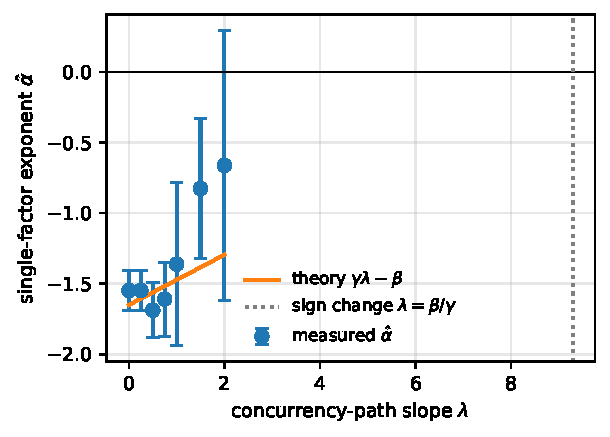
\includegraphics[width=\textwidth]{figures/fig_confounding}
\caption{Виміряні $\ahat$ (точки) проти аналітичного $\gamma\lambda-\beta$
(лінія) (Пропозиція~\ref{prop:identifiability}); передбачена зміна знака при
$\lambda=\resLambda$, поза перевіреними шляхами}
\label{fig:confounding}
\end{minipage}\hfill
\begin{minipage}[t]{0.31\textwidth}
\centering
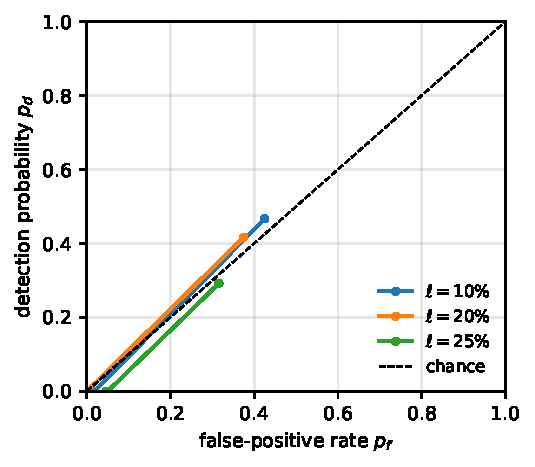
\includegraphics[width=\textwidth]{figures/fig_roc}
\caption{Виміряна ROC детектора (AUC$\,=\,\resAuc$, майже випадковий рівень);
детекційне обмеження з ним невиконуване}
\label{fig:roc}
\end{minipage}\hfill
\begin{minipage}[t]{0.32\textwidth}
\centering
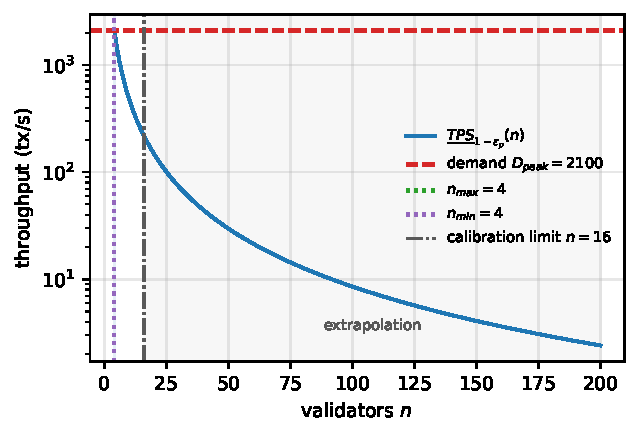
\includegraphics[width=\textwidth]{figures/fig_window}
\caption{Сценарій~A: нижня межа PI пропускної здатності vs.\ $\n$ при
$\kappaScale=\resKappa$; вікно $[\resNminCase,\resNmaxCase]$; штрихпунктир:
межа калібрування $\n=\resNmaxMeasured$}
\label{fig:window}
\end{minipage}
\end{figure}

\emph{X2 --- режим квот.}
X2 вимірює $\n\in\{4,7,13\}$ при $\cc=16$. Частковий $F$-тест взаємодії
квота\,$\times\log\n$ відхиляє спільний нахил ($p=\resQinvP$): $\beta$
дорівнює $\resBetaQlow$ і $\resBetaQmid$ при $\q=0.20,0.25$, але
$\resBetaQhigh$ при $\q=0.33$. У комірках $\q=0.33$ пропускна здатність при
$\n=4$ вже не зростає з квотою ($\resTpsQlowNfour$, $\resTpsQmidNfour$,
$\resTpsQhighNfour$~TPS), що вказує на не-CPU стелю, яка порушує
Припущення~\ref{as:separable}, а при $\n=13$ резервація $\approx4.3$ ядра
перевищує ємність хоста, тобто виходить за Означення~\ref{def:rnm}. Отже,
\RNM{} стабілізує $\beta$ за фіксованої квоти в CPU-обмеженому режимі, але не
робить його незалежним від квоти; коефіцієнти звітовано при $\q=0.25$.

\emph{X4 --- затримка.}
На власній сітці ($\n\in\{7,13\}$, $\cc=16$, $\q=0.25$) X4 дає
$\beta=\resBetaRttZero$ при $0$~мс і $\resBetaRttHigh$ при $200$~мс RTT
($\Delta\beta=\resDeltaBetaRtt$). Базове значення --- двоточковий нахил за
чотирма прогонами; воно узгоджується зі спільною підгонкою $\beta=\resBeta$ у
межах $1.3$ стандартної похибки. Проміжні RTT немонотонні
(табл.~\ref{tab:results}), тож X4 показує напрям і приблизну величину
WAN-штрафу, а не закон залежності від затримки.

\emph{X5 --- детектор.}
За $\resDetRuns$ прогонами з ін'єкцією відмов об'єднана ROC має
AUC$\,=\,\resAuc$ (рис.~\ref{fig:roc}, майже випадковий рівень); $\rho$ з цих
прогонів не ідентифікується і покладається рівним~$0$. За цих частот
детекційне обмеження невиконуване і його послаблено (не застосовується)
(підрозділ~\ref{sec:detection}).

\begin{table}[!t]
\centering
\caption{Калібровані параметри, перевірка квот, детектор і покриття
(досліджене розгортання)}
\label{tab:results}
\scriptsize
\begin{tabular}{lll}
\headline
Величина & Оцінка & Примітка \\
\headline
$\Tzero$; $\beta$; $\gamma$ &
  $\resTzero$; $\resBeta\pm\resBetaSE$; $\resGamma\pm\resGammaSE$ &
  двофакторна \\
$\csat$, $\theta$; $\hat\sigma$ & $\resCsat$, $\resTheta$; $\resSigmaRes$ &
  насичення / залишок \\
$\ahat$ при $\lambda=0,1,2$ &
  $\resAlphaHatLzero$, $\resAlphaHatLone$, $\resAlphaHatLtwo$ &
  X3b \\
$\beta$ при $q=0.20,0.25,0.33$ &
  $\resBetaQlow$, $\resBetaQmid$, $\resBetaQhigh$ &
  X2, $p=\resQinvP$ \\
$\beta$ при RTT $0,25,50,100,200$~мс &
  $\resBetaRttZero$, $\resBetaRttTwentyFive$, $\resBetaRttFifty$,
  $\resBetaRttHundred$, $\resBetaRttHigh$ &
  X4, $\n\in\{7,13\}$ \\
$\hat p_{d}$, $\hat p_{f}$ (частоти позначення); $J$; AUC &
  $\resPd$, $\resPf$; $\resYouden$; $\resAuc$ &
  X5, поріг $\resDetectorThr$ \\
покриття $90\%$/$95\%$ &
  $\resCovHitsNinety/\resHoldoutRuns$, $\resCovHitsNinetyFive/\resHoldoutRuns$ &
  підгонка $\n\le\resCalibMaxN$; hold-out $\resHoldoutN$ \\
\headline
\end{tabular}
\end{table}

\emph{X7/X8 --- покриття, порівняння та абляція.}
Окрема переоцінка на $\resCalibRuns$ прогонах без відмов з
$\n\le\resCalibMaxN$, яка не бачить відкладених прогонів, дає інтервали, що
покривають $\resCovHitsNinety$ і $\resCovHitsNinetyFive$ з $\resHoldoutRuns$
прогонів ($\resHoldoutN$) на рівнях $90\%$ і $95\%$. Перевірка груба
(більшість прогонів при $\n=13$, квоти X2 об'єднано, біноміальна похибка
$\approx6$~п.п.; $\n=11$ не має вигляду $3f+1$) і стосується процедури
інтервалів, а не основного $\beta=\resBeta$.
Позавибіркова log-RMSE для лінійного / однофакторного / USL~\cite{gunther2007} /
двофакторного прогнозів становить $\resRmseLinear$, $\resRmseSingle$,
$\resRmseUsl$, $\resRmseOurs$; однофакторний прогноз тут трохи точніший лише
тому, що всі відкладені прогони мають $\cc=16$. Відносні вартості визначення
розміру: $\resCostLinear$, $\resCostSingle$, $\resCostUsl$, $\resCostOurs$.

\section{Застосування, наслідки та обмеження}
\label{sec:case}

\subsection{Застосування та аналіз сценаріїв}

Інстанціюємо Задачу~\ref{prob:sizing} на $\approx3\times10^{7}$ бюлетенів за
дванадцять годин: середнє навантаження $\approx694$~TPS і, за припущеного
пік-фактора $\approx3$ (не виміряний профіль), пікове
$\Dpk=\resDemand$~TPS. Вимогу детекції --- скоординованої відмови з пропуском
транзакцій (coordinated transaction-omission fault) частки $\phi=0.2$ протягом
однієї епохи --- невиконувана, тож її послаблено (не застосовується;
підрозділ~\ref{sec:detection}), і $\nmin=4$. Прогони на CI без відмов і без
емульованої затримки фіксують не більше $\approx\resTpsMaxMeasured$~TPS (при
$\n=\resTpsMaxN$, $\cc=\resTpsMaxC$, $\q=\resTpsMaxQ$); модель працює в
одиницях \RNM{} $\TPSn=\TPS/\q$ (пропускна здатність на ядро квоти
валідатора), і за Припущенням~\ref{as:separable} масштаб $\kappaScale$ --- це
кількість ядер на валідатор у цільовому класі обладнання. Лінійність
пропускної здатності за квотою --- головне припущення й основний ризик
екстраполяції: $\kappaScale=\resKappa$ ядра у $\approx\resKappaQuotaRatio$
разів перевищує калібровану $\q=0.25$, тоді як X2 уже при $\q=0.33$ показує,
що пропускна здатність перестає зростати. Тож $\kappaScale$ --- вимога до
обладнання, яку треба перевірити на цільовому залізі, а не виміряна
можливість. За вільного
$\kappaScale$ Задача~\ref{prob:sizing} бере
\begin{equation}
\kappaScale^{\star}
=\frac{\Dpk}{\underline{\TPSn}_{1-\epsp}(4,\cc^{\star})},
\label{eq:kappa}
\end{equation}
мінімальний масштаб, при якому нижня межа прогнозного інтервалу при $\n=4$
досягає $\Dpk$.

\paragraph{Сценарій A (базовий).}
Підстановка каліброваних коефіцієнтів
($\beta=\resBeta$, $\gamma=\resGamma$) при $\cc^{\star}=\resCstar$ дає
$\kappaScale=\resKappa$ (ядер на валідатор) і вікно допустимості
$[\resNminCase,\resNmaxCase]$ з $\nopt=\resNoptCase$
(Пропозиція~\ref{prop:window}; рис.~\ref{fig:window}). Єдина допустима
кількість --- наслідок побудови: $\kappaScale$ --- найменший масштаб, що
допускає $\n=4$, тож $h(4)=0$ і, при $\beta>0$, $\nmax=4$; інформативним
результатом є саме $\kappaScale$. ($\cc^{\star}$ максимізує підігнану $\gfun$
поза сіткою МНК $\cc\le\resCalibCmax$; при $\cc=\resCalibCmax$
$\kappaScale=\resKappaCalibC$.)

\paragraph{Сценарії B і C (фіксований клас обладнання).}
Фіксуємо $\kappaScale=\resKappa$. Подвоєння $\Dpk$ дає $h(4)=-\log2<0$;
збільшення $\beta$ на WAN-приріст у межах X4 $\Delta\beta=\resDeltaBetaRtt$
знижує $h(4)$ на $\Delta\beta\log4$. Обидва вікна порожні
(Наслідок~\ref{cor:infeasible}), і додавання валідаторів не допомагає, бо
прогнозована пропускна здатність спадає з~$\n$. Обидва випливають з нульового
запасу в Сценарії~A; їхній зміст --- потрібний масштаб:
$\kappaScale=\resKappaDoubled$ і $\approx\resKappaWan$ для подвоєного попиту та
WAN відповідно.

Той самий робочий процес застосовується до реєстрів і ідентичності після
перекалібрування; обов'язкові вибори на блокчейні залишаються поза рекомендацією
\cite{springall2014,specter2020,park2021}.

\subsection{Наслідки}
\label{sec:discussion}

Підігнана пара $(\beta,\gamma)$ специфічна для Besu/QBFT і розгортання;
перенесення доречне лише тоді, коли шлях конкурентності, режим квот і клас RTT
збігаються з калібруванням, тоді як протокол \RNM{} і робочий процес
переносяться через перекалібрування. Бенчмарки мають звітувати $\lambda$ (або
$\lambda=0$), квоту на валідатор і клас RTT (Наслідок~\ref{cor:sign}).

\subsection{Обмеження}
\label{sec:limitations}

\emph{Клас відмов і детекція.} Зашифрований транспорт обмежує X5
omission/duplication, а отриманий детектор близький до випадкового; тож
детекційна частина задачі емпірично не задіяна, і демонстрація компромісу
«пропускна здатність --- детекція» потребує детектора з $J$, відділеним від
нуля.

\emph{Інфраструктура.} Чотириядерна CI з $\n\le\resNmaxMeasured$ ---
запланований субстрат; при $\n=\resNmaxMeasured$ резервація дорівнює чотирьом
ядрам хоста. Поза виміряними кількостями прогнози модель-базовані.

\section{Висновки}
\label{sec:conclusions}

\paragraph{Аналітичні результати.}
За ненасиченої двофакторної моделі з шумом нульового середнього і скінченної
дисперсії та зазначених припущень щодо шляху однофакторний показник МНК
задовольняє $\ahat_{m}\xrightarrow{\Prob}\gamma\lambda-\beta$
(Пропозиція~\ref{prop:identifiability}) --- зміщення через пропущену змінну.
Протилежні монотонні обмеження дають замкнене цілочислове вікно допустимості
(Пропозиція~\ref{prop:window}).

\paragraph{Експериментально підтримані спостереження.}
За \RNM{} на чотириядерній типовій CI $\beta=\resBeta\pm\resBetaSE$ і
$\gamma=\resGamma\pm\resGammaSE$ при $\q=0.25$; $\beta$ стабільний за
фіксованої квоти, але залежить від її рівня; повторне семплювання шляху
узгоджене з $\gamma\lambda-\beta$. Детектор близький до випадкового, тож вікно
визначає лише пропускна здатність. Подвоєний попит або WAN~$\beta$ потребує
$\kappaScale=\resKappaDoubled$ або $\approx\resKappaWan$ відповідно замість
$\resKappa$; ці значення спираються на неперевірену лінійність пропускної
здатності за квотою.
Числові результати специфічні для розгортання.

\paragraph{Інженерні наслідки.}
Внесок --- відтворювана методика ресурсно-нормованого калібрування та
планування потужності; компроміс «пропускна здатність --- детекція»
сформульовано, але з виміряним детектором не продемонстровано. Інші
розгортання потребують перекалібрування $(\beta,\gamma)$ і $(\pd,\pf,\rho)$ зі
збереженням того самого робочого процесу та публічних артефактів.

\subsection*{Конфлікт інтересів}
Автори заявляють про відсутність конфлікту інтересів.

\subsection*{Фінансування}
Дослідження виконано без фінансової підтримки.

\subsection*{Доступність даних}
Означення робочого процесу, генератори, код ін'єкції відмов і аналізу та сирі
артефакти доступні за адресою
\url{https://github.com/bpenyak/Resource_Normalized_Scaling_Laws_for_Byzantine_Consensus}.

\subsection*{Використання штучного інтелекту}
AI-допоміжні інструменти використано для мовного редагування та верстки. Усі
наукові результати, доведення, дизайн і аналіз виконані авторами.

\subsection*{Внесок авторів}
\textbf{Пеняк Б.\,О.}: концептуалізація, методологія, формальний аналіз,
програмне забезпечення, дослідження, курація даних, написання --- первинний
текст, візуалізація.
\textbf{Любінський Б.\,Б.}: наукове керівництво, валідація, написання ---
рецензування та редагування.


%%%%%%%%%%%%%%%%%%%%%%%%%%%%%%%%%%%%%%%%%%%%%%%%%%%%%%%%%%%%%%%%%%%%%%%%%%%%%%%
%% bib/references.tex
%% MMC.sty redefines `thebibliography'. Do NOT use bibtex / biblatex.
%% Count: 29 entries (requirement: >= 25).
%% Every entry ends with a resolvable \url{...} (DOI preferred; open PDF/arXiv
%% when the publisher blocks automated DOI resolution).
%%%%%%%%%%%%%%%%%%%%%%%%%%%%%%%%%%%%%%%%%%%%%%%%%%%%%%%%%%%%%%%%%%%%%%%%%%%%%%%

\begin{thebibliography}{28}

%------------------------------------------------------- BFT consensus
\bibitem{castro1999}
Castro M., Liskov B. Practical Byzantine fault tolerance. Proceedings of the
Third Symposium on Operating Systems Design and Implementation (OSDI). 173--186
(1999).
\url{https://www.usenix.org/conference/osdi-99/practical-byzantine-fault-tolerance}

\bibitem{lamport1982}
Lamport L., Shostak R., Pease M. The Byzantine generals problem. ACM
Transactions on Programming Languages and Systems. \textbf{4} (3), 382--401
(1982).
\url{https://doi.org/10.1145/357172.357176}

\bibitem{dwork1988}
Dwork C., Lynch N., Stockmeyer L. Consensus in the presence of partial
synchrony. Journal of the ACM. \textbf{35} (2), 288--323 (1988).
\url{https://doi.org/10.1145/42282.42283}

\bibitem{yin2019}
Yin M., Malkhi D., Reiter M.~K., Gueta G.~G., Abraham I. HotStuff: BFT consensus
with linearity and responsiveness. Proceedings of the ACM Symposium on
Principles of Distributed Computing (PODC). 347--356 (2019).
\url{https://doi.org/10.1145/3293611.3331591}
\url{https://arxiv.org/abs/1803.05069}

\bibitem{buchman2016}
Buchman E. Tendermint: Byzantine fault tolerance in the age of blockchains.
Master's thesis, University of Guelph (2016).
\url{https://hdl.handle.net/10214/9769}

\bibitem{gilad2017}
Gilad Y., Hemo R., Micali S., Vlachos G., Zeldovich N. Algorand: scaling
Byzantine agreements for cryptocurrencies. Proceedings of the 26th Symposium on
Operating Systems Principles (SOSP). 51--68 (2017).
\url{https://doi.org/10.1145/3132747.3132757}
\url{https://arxiv.org/abs/1607.01341}

\bibitem{miller2016}
Miller A., Xia Y., Croman K., Shi E., Song D. The honey badger of BFT protocols.
Proceedings of the ACM SIGSAC Conference on Computer and Communications Security
(CCS). 31--42 (2016).
\url{https://doi.org/10.1145/2976749.2978399}
\url{https://eprint.iacr.org/2016/199}

\bibitem{vukolic2015}
Vukoli\'{c} M. The quest for scalable blockchain fabric: proof-of-work vs.\ BFT
replication. Open Problems in Network Security. IFIP AICT, vol.~468. Springer.
112--125 (2015).
\url{https://doi.org/10.1007/978-3-319-39028-4_9}

%--------------------------------------------------------- benchmarking
\bibitem{androulaki2018}
Androulaki E., et al. Hyperledger Fabric: a distributed operating system for
permissioned blockchains. Proceedings of the Thirteenth EuroSys Conference.
30:1--30:15 (2018).
\url{https://doi.org/10.1145/3190508.3190538}
\url{https://arxiv.org/abs/1801.10228}

\bibitem{thakkar2018}
Thakkar P., Nathan S., Viswanathan B. Performance benchmarking and optimizing
Hyperledger Fabric blockchain platform. 26th IEEE International Symposium on
Modeling, Analysis, and Simulation of Computer and Telecommunication Systems
(MASCOTS). 264--276 (2018).
\url{https://doi.org/10.1109/MASCOTS.2018.00034}

\bibitem{dinh2017}
Dinh T.~T.~A., Wang J., Chen G., Liu R., Ooi B.~C., Tan K.-L. BLOCKBENCH: a
framework for analyzing private blockchains. Proceedings of the ACM
International Conference on Management of Data (SIGMOD). 1085--1100 (2017).
\url{https://doi.org/10.1145/3035918.3064033}
\url{https://arxiv.org/abs/1703.04057}

\bibitem{sousa2018}
Sousa J., Bessani A., Vukoli\'{c} M. A Byzantine fault-tolerant ordering service
for the Hyperledger Fabric blockchain platform. 48th IEEE/IFIP International
Conference on Dependable Systems and Networks (DSN). 51--58 (2018).
\url{https://doi.org/10.1109/DSN.2018.00018}

%------------------------------------------------------- scaling laws
\bibitem{amdahl1967}
Amdahl G.~M. Validity of the single processor approach to achieving large scale
computing capabilities. Proceedings of the AFIPS Spring Joint Computer
Conference. 483--485 (1967).
\url{https://doi.org/10.1145/1465482.1465560}

\bibitem{gustafson1988}
Gustafson J.~L. Reevaluating Amdahl's law. Communications of the ACM.
\textbf{31} (5), 532--533 (1988).
\url{https://doi.org/10.1145/42411.42415}

\bibitem{gunther2007}
Gunther N.~J. Guerrilla capacity planning: a tactical approach to planning for
highly scalable applications and services. Springer (2007).
\url{https://doi.org/10.1007/978-3-540-31010-5}

%----------------------------------------------- concentration, statistics
\bibitem{hoeffding1963}
Hoeffding W. Probability inequalities for sums of bounded random variables.
Journal of the American Statistical Association. \textbf{58} (301), 13--30
(1963).
\url{https://doi.org/10.1080/01621459.1963.10500830}

\bibitem{kish1965}
Kish L. Survey sampling. John Wiley \& Sons, New York (1965).
\url{https://archive.org/details/surveysampling00kish}
\bibitem{boucheron2013}
Boucheron S., Lugosi G., Massart P. Concentration inequalities: a nonasymptotic
theory of independence. Oxford University Press (2013).
\url{https://doi.org/10.1093/acprof:oso/9780199535255.001.0001}

\bibitem{efron1993}
Efron B., Tibshirani R.~J. An introduction to the bootstrap. Chapman and Hall
(1993).
\url{https://doi.org/10.1201/9780429246593}

\bibitem{seber2003}
Seber G.~A.~F., Wild C.~J. Nonlinear regression. Wiley (2003).
\url{https://doi.org/10.1002/0471725315}

\bibitem{wooldridge2010}
Wooldridge J.~M. Econometric analysis of cross section and panel data.
2nd ed. MIT Press (2010).
\url{https://mitpress.mit.edu/9780262232586/}

%------------------------------------ optimization under uncertainty
\bibitem{charnes1959}
Charnes A., Cooper W.~W. Chance-constrained programming. Management Science.
\textbf{6} (1), 73--79 (1959).
\url{https://doi.org/10.1287/mnsc.6.1.73}

\bibitem{nemirovski2007}
Nemirovski A., Shapiro A. Convex approximations of chance constrained programs.
SIAM Journal on Optimization. \textbf{17} (4), 969--996 (2006/2007).
\url{https://doi.org/10.1137/050622328}
\url{https://optimization-online.org/wp-content/uploads/2004/12/1033.pdf}

%--------------------------------------------- e-governance, e-voting
\bibitem{springall2014}
Springall D., Finkenauer T., Durumeric Z., Kitcat J., Hursti H., MacAlpine M.,
Halderman J.~A. Security analysis of the Estonian internet voting system.
Proceedings of the ACM SIGSAC Conference on Computer and Communications Security
(CCS). 703--715 (2014).
\url{https://doi.org/10.1145/2660267.2660315}
\url{https://jhalderm.com/pub/papers/ivoting-ccs14.pdf}

\bibitem{specter2020}
Specter M.~A., Koppel J., Weitzner D. The ballot is busted before the
blockchain: a security analysis of Voatz. Proceedings of the 29th USENIX
Security Symposium. 1535--1553 (2020).
\url{https://www.usenix.org/system/files/sec20-specter.pdf}

\bibitem{park2021}
Park S., Specter M., Narula N., Rivest R.~L. Going from bad to worse: from
internet voting to blockchain voting. Journal of Cybersecurity. \textbf{7} (1),
tyaa025 (2021).
\url{https://doi.org/10.1093/cybsec/tyaa025}

%------------------------------------------------------------- tooling
\bibitem{besu}
Hyperledger Besu documentation. Hyperledger Foundation.
\url{https://github.com/hyperledger/besu}
\url{https://www.hyperledger.org/use/besu}

%--------------------------------------------------------- own prior work
\bibitem{peniak2026a}
Peniak B.~O., Liubinskiy B.~B., Solomka I.~R. Minimal-sample performance
prediction for Byzantine consensus: the $\alpha$-calibration method.
Mathematical Modeling and Computing. (accepted; to appear) (2026).
\url{https://science.lpnu.ua/mmc}

\bibitem{peniak2026b}
Peniak B.~O., Liubinskiy B.~B. Adaptive hybrid consensus mechanism for
blockchain-based \mbox{e-governance}: a machine learning approach. Scientific Bulletin
of Uzhhorod University. Series of Mathematics and Informatics. \textbf{49} (2),
255--261 (2026).
\url{https://doi.org/10.24144/2616-7700.2026.49(2).255-261}

\end{thebibliography}


\newpage
\English
\noindent\textbf{\Large Abstract (English)}\\[1ex]
Peniak B.\,O., Liubinskiy B.\,B.\\[0.5ex]
{\small Lviv Polytechnic National University,
12 S.~Bandera str., 79013, Lviv, Ukraine}\\[1.5ex]
Sizing a permissioned BFT validator set for \mbox{e-governance} trades
consensus throughput, which falls with~$\n$, against fault-detection power,
which rises with it. We propose resource-normalized measurement with a fixed
per-validator CPU quota; show that, in the unsaturated bi-factor model with
zero-mean noise, the single-factor OLS exponent tends to
$\gamma\lambda-\beta$ (an \mbox{omitted-variable} bias); and formulate
chance-constrained sizing with feasible set $[\nmin,\nmax]$. On four-core
public CI ($\n\le\resNmaxMeasured$) the exponent is stable at a fixed quota but
quota-dependent; the measured detector is near chance (AUC$\,=\,\resAuc$), so
the detection constraint is relaxed (not enforced) and throughput alone sets
the window. Coefficients are deployment-specific.

\end{document}
